\subsection{Mise en rampe}
\label{subsec:mise_en_rampe}

Enfin, nous détaillons l'intégration finale de la fusée sur la rampe de lancement. Nous prévoyons une installation
en plusieurs étapes :
\begin{itemize}
    \item Le positionnement du premier étage via ses deux patins (un au niveau du rétrein et le second au niveau des aérofreins),
    \item Le positionnement du second étage avec son extension de rampe avec sa cale d'arrêt,
    \item L'insertion du Pro24-6G,
    \item Le couplage des deux vecteurs,
    \item Le retrait de l'extension de rampe du second étage,
    \item L'élévation de la rampe pour les opérations pyrotechniques du Pro54-5G
\end{itemize}

Comme nous possédons quatre ailerons par étage, nous avons décallé notre jeu d'ailerons supérieur de 15°, ce qui nous donne un
angle maximal entre les deux étages de 70° pour le passage de la rampe. Cette contrainte visible ci-dessous devra être validée
concernant le treillis de la rampe qui doit passer dans cet intervale.
\begin{figure}[h!] 
    \centering 
    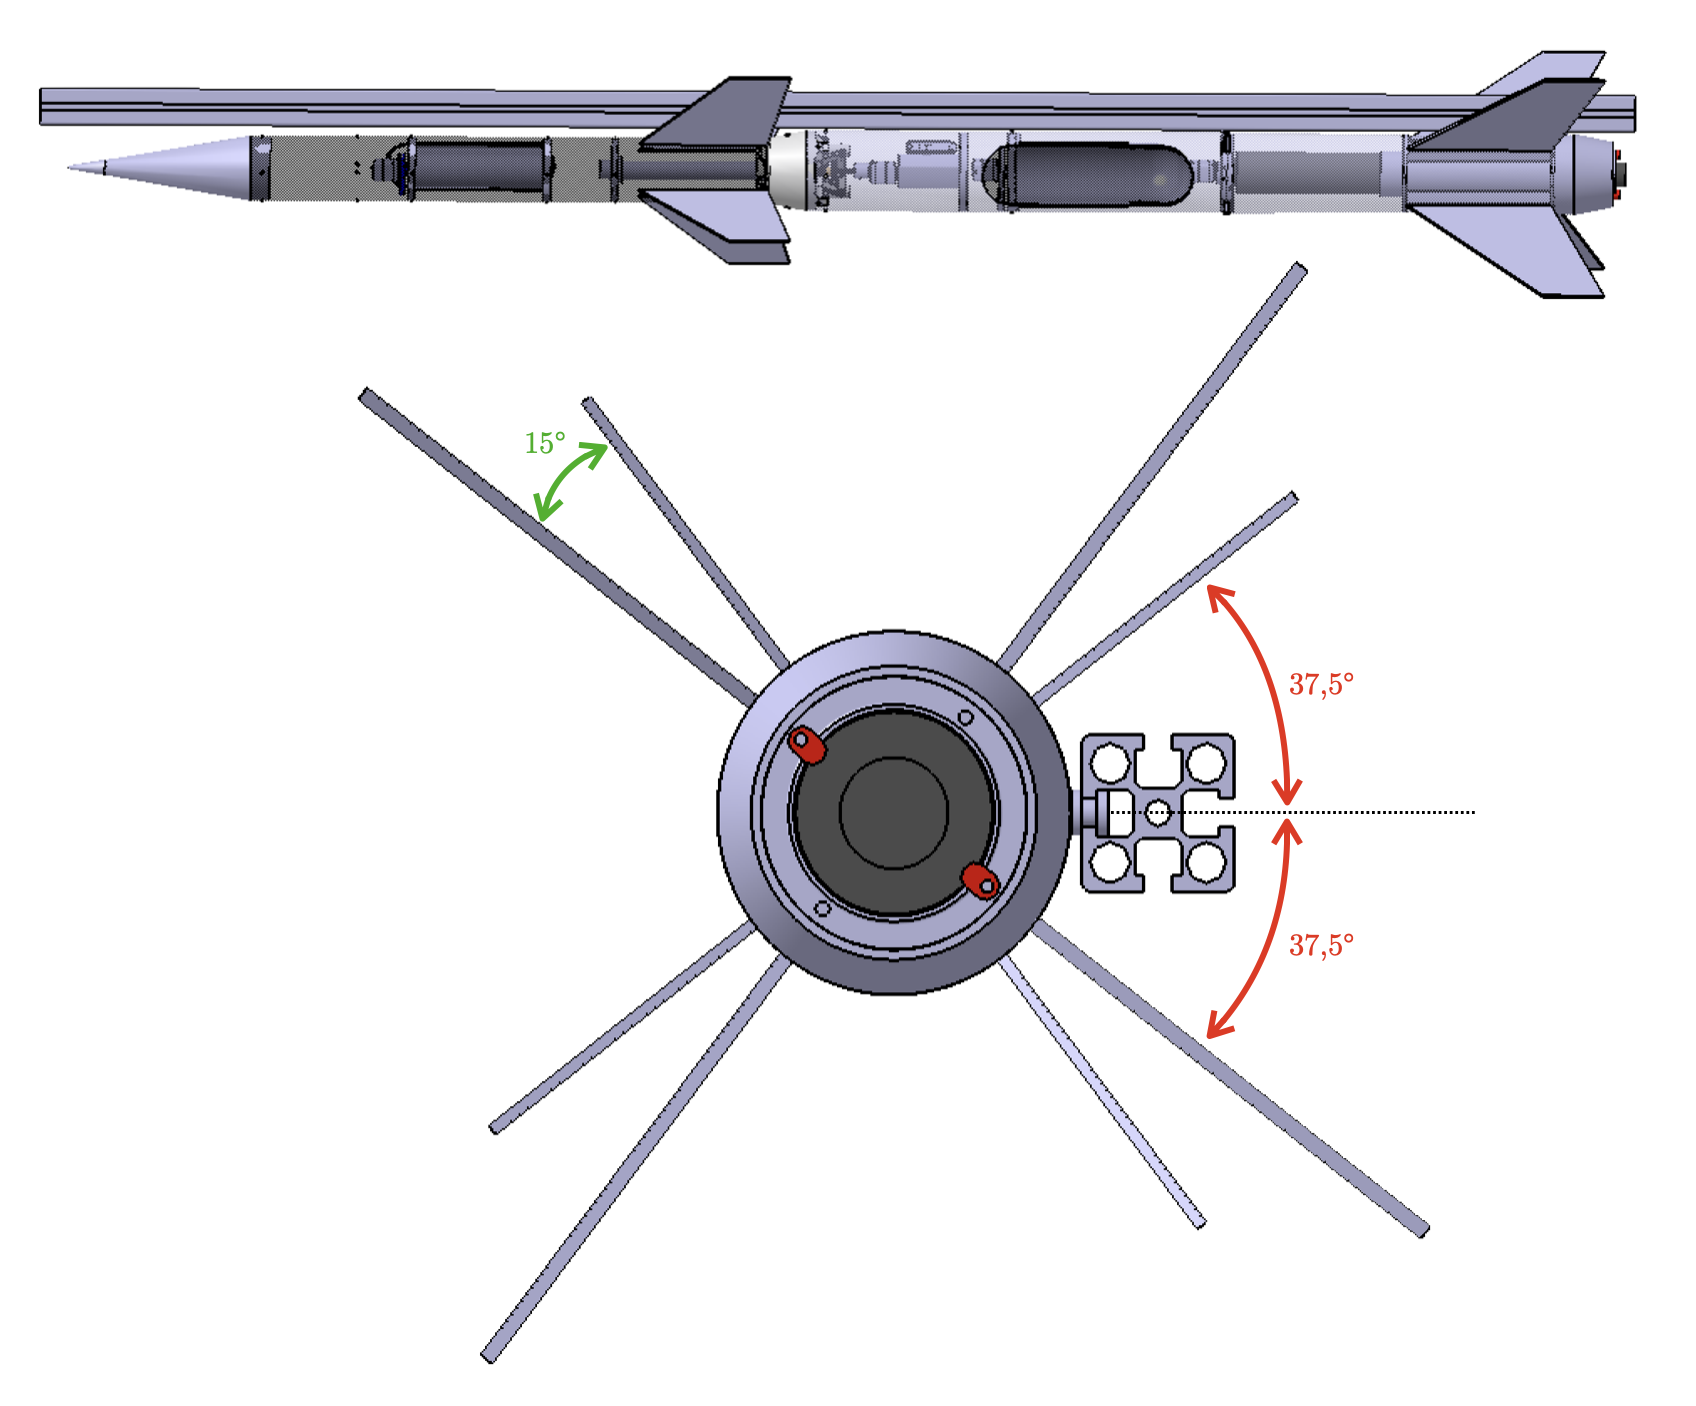
\includegraphics[width=0.8\textwidth]{figures/meca/mise_en_rampe.png} 
    \caption{Angles entre les ailerons proches de la rampe sur la configuration de mise en rampe} 
    \label{fig:para_etage2} 
\end{figure}